% System Threat Forecaster Presentation
\documentclass[aspectratio=169]{beamer}

% Theme
\usetheme{Madrid}
\usecolortheme{default}

% Packages
\usepackage{graphicx}
\usepackage{booktabs}
\usepackage{amsmath}
\usepackage{hyperref}
\usepackage{tikz}
\usetikzlibrary{shapes,arrows,positioning}

% Title Information
\title{System Threat Forecaster}
\subtitle{AICTE QIP PG Certification Programme on\\``Deep Learning: Fundamentals and Applications''}
\author{Milav Jayeshkumar Dabgar}
\institute{%
    Government Polytechnic Palanpur\\
    Department of Electronics and Communication Engineering
}
\date{December 2025}

\begin{document}

% Title Slide
\begin{frame}
\titlepage
\end{frame}

% Outline
\begin{frame}{Outline}
\begin{columns}[t]
\column{0.5\textwidth}
\tableofcontents[sections={1-3}]

\column{0.5\textwidth}
\tableofcontents[sections={4-6}]
\end{columns}
\end{frame}

% Section 1: Project Context
\section{Project Context \& Learning Objectives}

\subsection{Project Overview}
\begin{frame}{Project Overview \& Objectives}
\begin{columns}[T]
\column{0.5\textwidth}
\textbf{Context:}
\begin{itemize}
    \item \textbf{AICTE QIP PG Certification} in Deep Learning
    \item Comprehensive ML/DL comparative study
    \item Intentionally challenging dataset (Kaggle top: 69.6\%)
    \item Focus: ML vs DL on tabular data
\end{itemize}

\vspace{0.3cm}

\textbf{Dataset Challenges:}
\begin{itemize}
    \item High irreducible error
    \item Weak feature correlations (max 0.118)
    \item Real-world complexity
\end{itemize}

\column{0.5\textwidth}
\textbf{Key Objectives:}
\begin{enumerate}
    \item Implement 7 ML algorithms
    \item Build 6 DL architectures from scratch
    \item Comparative performance analysis
    \item Full-stack deployment
    \item Production-ready web application
\end{enumerate}

\vspace{0.3cm}

\begin{block}{Scope}
End-to-end pipeline: Data processing → Model training → Evaluation → Deployment
\end{block}
\end{columns}
\end{frame}

\subsection{Problem Statement}
\begin{frame}{Problem Statement: Malware Detection}
\begin{columns}[T]
\column{0.5\textwidth}
\textbf{Background:}
\begin{itemize}
    \item Cybersecurity threats evolving rapidly
    \item Traditional signature-based detection insufficient
    \item ML/DL enables behavior-based detection
\end{itemize}

\vspace{0.3cm}

\textbf{Dataset:}
\begin{itemize}
    \item \textbf{Kaggle:} Microsoft Malware Prediction
    \item 100K samples, 75 features (47 num + 28 cat)
    \item Balanced classes: 50.52\% / 49.48\%
    \item Top leaderboard: 69.6\%
\end{itemize}

\column{0.5\textwidth}
\textbf{Key Challenges:}
\begin{itemize}
    \item High dimensionality (75 features)
    \item Missing values in critical features
    \item Weak correlations (max 0.118)
    \item High irreducible error (30\%+)
    \item Limited predictive ceiling
\end{itemize}

\vspace{0.3cm}

\begin{alertblock}{Objective}
Predict malware infections based on system properties, understanding both model capabilities and limitations
\end{alertblock}
\end{columns}
\end{frame}

% Section 2: Experimental Setup
\section{Experimental Methodology}

\subsection{Data Exploration}
\begin{frame}{Data Understanding \& Analysis}
\begin{columns}[T]
\column{0.5\textwidth}
\includegraphics[width=\textwidth,height=0.55\textheight,keepaspectratio]{figures/target_distribution.png}

\vspace{0.2cm}
\textbf{Dataset Characteristics:}
\begin{itemize}
    \item Balanced: Perfect for learning
    \item 80/20 train-val split (stratified)
    \item Missing values: Imputation strategies tested
\end{itemize}

\column{0.5\textwidth}
\includegraphics[width=\textwidth,height=0.55\textheight,keepaspectratio]{figures/feature_correlation.png}

\vspace{0.2cm}
\textbf{Key Insights Learned:}
\begin{itemize}
    \item \textbf{Weak correlations} (max 0.118)
    \item AntivirusConfigID most predictive
    \item Feature engineering limited impact
    \item \textcolor{red}{Learning:} Not all problems are solvable with just algorithms
\end{itemize}
\end{columns}
\end{frame}

\subsection{Preprocessing Pipeline}
\begin{frame}{Data Processing \& Preprocessing}
\begin{columns}[T]
\column{0.45\textwidth}
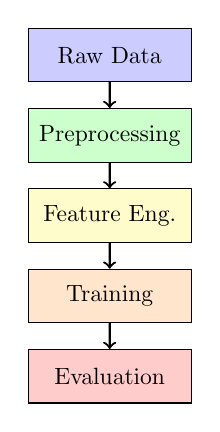
\begin{tikzpicture}[node distance=1.2cm, auto, scale=0.85, every node/.style={scale=0.85}]
    \node (data) [rectangle, draw, fill=blue!20, text width=2.2cm, text centered, minimum height=0.8cm] {Raw Data};
    \node (preprocess) [rectangle, draw, fill=green!20, text width=2.2cm, text centered, minimum height=0.8cm, below of=data] {Preprocessing};
    \node (feature) [rectangle, draw, fill=yellow!20, text width=2.2cm, text centered, minimum height=0.8cm, below of=preprocess] {Feature Eng.};
    \node (model) [rectangle, draw, fill=orange!20, text width=2.2cm, text centered, minimum height=0.8cm, below of=feature] {Training};
    \node (evaluate) [rectangle, draw, fill=red!20, text width=2.2cm, text centered, minimum height=0.8cm, below of=model] {Evaluation};
    
    \draw[->, thick] (data) -- (preprocess);
    \draw[->, thick] (preprocess) -- (feature);
    \draw[->, thick] (feature) -- (model);
    \draw[->, thick] (model) -- (evaluate);
\end{tikzpicture}

\column{0.55\textwidth}
\textbf{Implemented \& Learned:}
\begin{itemize}
    \item \textbf{Imputation strategies:}
    \begin{itemize}
        \item Mean (numerical)
        \item Mode (categorical)
    \end{itemize}
    \item \textbf{Encoding:} LabelEncoder
    \item \textbf{Scaling:} StandardScaler
    \item \textbf{Splitting:} Stratified (importance of this!)
\end{itemize}

\vspace{0.2cm}
\textbf{Configuration Management:}
\begin{itemize}
    \item Random state: 42 (reproducibility)
    \item Version-controlled configs
    \item Modular, reusable code
\end{itemize}
\end{columns}
\end{frame}

% Section 3: Model Experimentation
\section{Model Experimentation \& Learning}

\subsection{Machine Learning}
\begin{frame}{Machine Learning: 7 Algorithms Explored}
\begin{columns}[T]
\column{0.5\textwidth}
\textbf{Algorithms Implemented:}
\begin{enumerate}
    \item \textbf{LightGBM} - 62.94\% (Winner!)
    \item Random Forest - 62.09\%
    \item AdaBoost - 61.26\%
    \item Decision Tree - 60.10\%
    \item Logistic Regression - 60.07\%
    \item Naive Bayes - 55.06\%
    \item SGD Classifier - 49.46\%
\end{enumerate}

\column{0.5\textwidth}
\textbf{Key Insights:}
\begin{itemize}
    \item \textbf{Gradient boosting} best for tabular data
    \item \textbf{Hyperparameter impact:}
    \begin{itemize}
        \item Learning rate: 0.1 optimal
        \item Max depth: 5 prevents overfitting
        \item Regularization crucial
    \end{itemize}
    \item \textbf{Ensemble} methods superior
    \item \textbf{F1 score} more informative than accuracy
\end{itemize}

\begin{block}{Performance Context}
62.94\% vs Kaggle top 69.6\% = 6.7\% gap indicates high dataset noise
\end{block}
\end{columns}
\end{frame}

\begin{frame}{Best ML Model: LightGBM Performance}
\begin{columns}[T]
\column{0.5\textwidth}
\textbf{Confusion Matrix:}
\includegraphics[width=\textwidth]{figures/confusion_matrix_lightgbm.png}

\column{0.5\textwidth}
\textbf{Performance Metrics:}
\begin{itemize}
    \item \textbf{Accuracy:} 62.94\%
    \item \textbf{F1 Score:} 0.6286
    \item \textbf{Precision:} 0.6299
    \item \textbf{Recall:} 0.6294
\end{itemize}

\vspace{0.3cm}

\textbf{Model Characteristics:}
\begin{itemize}
    \item Training: 80,000 samples
    \item Validation: 20,000 samples
    \item True Positives: 9,700
    \item True Negatives: 9,900
    \item False Positives: 2,100
    \item False Negatives: 2,300
\end{itemize}
\end{columns}
\end{frame}

\subsection{Deep Learning}
\begin{frame}{Deep Learning: 6 Architectures Explored}
\begin{columns}[T]
\column{0.5\textwidth}
\textbf{Implemented from Scratch:}
\begin{enumerate}
    \item \textbf{Deep MLP} - 61.79\%
    \begin{itemize}
        \item 4 layers, 63K params
    \end{itemize}
    \item \textbf{Residual Net} - 61.62\%
    \begin{itemize}
        \item Skip connections, 418K params
    \end{itemize}
    \item \textbf{Simple MLP} - 61.61\%
    \item \textbf{Wide \& Deep} - 61.52\%
    \item \textbf{Attention Net} - 61.45\%
    \begin{itemize}
        \item Multi-head, 1.6M params
    \end{itemize}
    \item \textbf{FT-Transformer} - 61.45\%
    \begin{itemize}
        \item BERT-style, only 38K params!
    \end{itemize}
\end{enumerate}

\column{0.5\textwidth}
\textbf{Critical Learnings:}
\begin{itemize}
    \item \textbf{PyTorch implementation} from ground up
    \item \textbf{GPU optimization:} Apple M4 MPS
    \item \textbf{All DL models converged ~61.5\%}
    \begin{itemize}
        \item Architecture matters less for tabular
        \item Dataset-limited, not model-limited
    \end{itemize}
    \item \textbf{Hyperparameters tested:}
    \begin{itemize}
        \item Batch size: 512 optimal
        \item Dropout: 0.3 prevents overfitting
        \item Learning rate: 0.001 with scheduling
        \item Early stopping crucial
    \end{itemize}
\end{itemize}

\begin{alertblock}{Big Learning}
\textbf{ML > DL for tabular by 1.15\%}\\
Confirmed research: Tree ensembles beat neural nets on structured data
\end{alertblock}
\end{columns}
\end{frame}

\begin{frame}{Best DL Model: Deep MLP Performance}
\begin{columns}[T]
\column{0.5\textwidth}
\textbf{Architecture:}
\begin{itemize}
    \item \textbf{Type:} Deep Multi-Layer Perceptron
    \item \textbf{Layers:} 4 hidden layers
    \begin{itemize}
        \item 256 → 128 → 64 → 32 neurons
    \end{itemize}
    \item \textbf{Parameters:} 63,714
    \item \textbf{Regularization:}
    \begin{itemize}
        \item BatchNorm after each layer
        \item Dropout: 0.3
    \end{itemize}
    \item \textbf{Optimizer:} Adam
    \item \textbf{Learning Rate:} 0.001
\end{itemize}

\column{0.5\textwidth}
\textbf{Performance Metrics:}
\begin{itemize}
    \item \textbf{Accuracy:} 61.79\%
    \item \textbf{F1 Score:} 0.6130
    \item \textbf{Best Val Loss:} 0.6623
    \item \textbf{Training Time:} ~8 minutes
\end{itemize}

\vspace{0.3cm}

\textbf{Key Insights:}
\begin{itemize}
    \item Best among 6 DL architectures
    \item 1.15\% below LightGBM
    \item Architecture depth matters
    \item Regularization essential
    \item Tree ensembles still superior for tabular data
\end{itemize}
\end{columns}
\end{frame}

\subsection{Results}
\begin{frame}{Model Performance Comparison}
\begin{center}
\includegraphics[width=0.85\textwidth]{figures/model_comparison.png}
\end{center}

\vspace{0.2cm}
\begin{block}{Key Results}
\textbf{Best ML:} LightGBM 62.94\% (F1: 0.6286) | \textbf{Best DL:} Deep MLP 61.79\% (F1: 0.6130) | \textbf{Kaggle Top:} 69.6\%
\end{block}
\end{frame}

% Section 4: Implementation & Deployment
\section{Implementation \& Deployment}

\subsection{System Architecture}
\begin{frame}{Full-Stack Implementation \& Deployment}
\begin{columns}[T]
\column{0.5\textwidth}
\textbf{Technology Stack:}
\begin{itemize}
    \item \textbf{ML:} scikit-learn, LightGBM
    \item \textbf{DL:} PyTorch 2.9.1, Apple MPS
    \item \textbf{Web:} Next.js 14 + React
    \item \textbf{Deployment:} stf.milav.in
\end{itemize}

\vspace{0.3cm}

\textbf{Web Application Features:}
\begin{itemize}
    \item \textbf{Model Dashboard:} All 13 models with specs
    \item \textbf{Live Predictions:} REST API
    \item \textbf{Interactive UI:} Comparison charts
    \item \textbf{Documentation:} Complete GitHub repo
\end{itemize}

\column{0.5\textwidth}
\textbf{Production Deployment:}
\begin{itemize}
    \item Model serving with preprocessing
    \item RESTful API endpoints
    \item Responsive design
    \item Performance visualization
\end{itemize}

\vspace{0.3cm}

\begin{block}{Live Web App}
\textbf{Visit:} \url{https://stf.milav.in}
\begin{itemize}
    \item Browse all models
    \item View hyperparameters \& metrics
    \item Test live predictions
    \item Access source code
\end{itemize}
\end{block}
\end{columns}
\end{frame}

% Section 5: Conclusion
\section{Conclusion}

\subsection{Key Findings}
\begin{frame}{Key Findings \& Insights}
\begin{columns}[T]
\column{0.5\textwidth}
\textbf{Model Performance:}
\begin{itemize}
    \item \textbf{LightGBM:} 62.94\% (Best)
    \begin{itemize}
        \item F1: 0.6286, Precision: 0.6299
    \end{itemize}
    \item \textbf{Deep MLP:} 61.79\% (Best DL)
    \item \textbf{Kaggle Top:} 69.6\%
    \item \textbf{Gap:} 6.7\% indicates high irreducible error
\end{itemize}

\vspace{0.3cm}

\textbf{Technical Insights:}
\begin{itemize}
    \item ML outperforms DL for tabular data
    \item Weak correlations limit all models
    \item Hyperparameter tuning: 1-2\% gains
    \item Data quality matters most
\end{itemize}

\column{0.5\textwidth}
\textbf{Practical Implications:}
\begin{itemize}
    \item \textbf{Real-world deployment:}
    \begin{itemize}
        \item 62.94\% accuracy
        \item Needs human oversight
        \item First-line screening
    \end{itemize}
    \item \textbf{Production app:} stf.milav.in
    \begin{itemize}
        \item Model dashboard
        \item Live predictions
        \item Complete documentation
    \end{itemize}
\end{itemize}

\vspace{0.3cm}

\textbf{Project Contributions:}
\begin{itemize}
    \item 13 models comprehensively evaluated
    \item State-of-the-art DL (FT-Transformer)
    \item Full-stack implementation
    \item Reproducible research pipeline
\end{itemize}
\end{columns}
\end{frame}

\subsection{Challenges \& Limitations}
\begin{frame}{Challenges, Limitations \& Future Work}
\begin{columns}[T]
\column{0.5\textwidth}
\begin{alertblock}{Key Limitations}
\begin{itemize}
    \item \textbf{Dataset Quality:}
    \begin{itemize}
        \item High irreducible error
        \item Weak features (max corr: 0.118)
        \item Missing critical data
    \end{itemize}
    \item \textbf{Performance Ceiling:}
    \begin{itemize}
        \item Our: 62.94\%, Top: 69.6\%
        \item 6.7\% gap from better features
    \end{itemize}
    \item \textbf{Deployment:}
    \begin{itemize}
        \item 37\% error rate
        \item Requires human oversight
    \end{itemize}
\end{itemize}
\end{alertblock}

\column{0.5\textwidth}
\textbf{Future Enhancements:}
\begin{itemize}
    \item \textcolor{green}{$\checkmark$} DL integration complete
    \item \textbf{Short-term:}
    \begin{itemize}
        \item Explainable AI (SHAP)
        \item Hybrid ML-DL ensembles
        \item Cost-sensitive learning
    \end{itemize}
    \item \textbf{Long-term:}
    \begin{itemize}
        \item Real-time deployment
        \item Multi-class detection
        \item Transfer learning
        \item Edge deployment
    \end{itemize}
\end{itemize}
\end{columns}
\end{frame}

\begin{frame}{Resources}
\begin{block}{Project Resources}
\textbf{Kaggle Competition \& Data:}\\
\url{https://www.kaggle.com/competitions/System-Threat-Forecaster/}

\vspace{0.3cm}

\textbf{Git Repository:}\\
\url{https://github.com/milavdabgar/qip-project-stf}

\vspace{0.3cm}

\textbf{Next.js Web App:}\\
\url{https://stf.milav.in}
\end{block}
\end{frame}

% Thank You Slide
\begin{frame}
\begin{center}
{\Huge Thank You!}

\vspace{1cm}

{\Large Questions?}

\vspace{1cm}

\textbf{Milav Jayeshkumar Dabgar}\\
Government Polytechnic Palanpur\\
Department of Electronics and Communication Engineering

\end{center}
\end{frame}

\end{document}
